\chapter{Model automobilu}
\label{sec:CarModel} \

V této kapitole je popsán model automobilu a jeho jednotlivé části.

Model automobilu je založen na platformě \textbf{Alamak}.
Platforma Alamak má 2 servomotory pro otáčení předních kol a 2 PWM motory pro řízení každého
zadního kola.

Platforma Alamak je řízená pomocí MCU FRDM-K66F\cite{frdmk66UserGuide} spolu
s modulem POLI-TFC přípojeným do GPIO pinů mikrokontroleru.
Detailní popis mikrokontroleru a modulu jsou v podkapitolách \ref{sec:FRDM-K66F} a \ref{sec:POLI-TFC}.

Pro komunikaci s platformou Alamak je použit WiFi Access Point, který je připojen k MCU
pomocí Ethernet portu.

Řádková kamera, která umístěna v přední části platformy, se používá pro získání obrazu drahy.

Vše je napojeno pomocí baterie typu NiMH o napětí 7.2V.

Celý model je zobrazen na obrázku.
\begin{figure}[h]
    \centering
    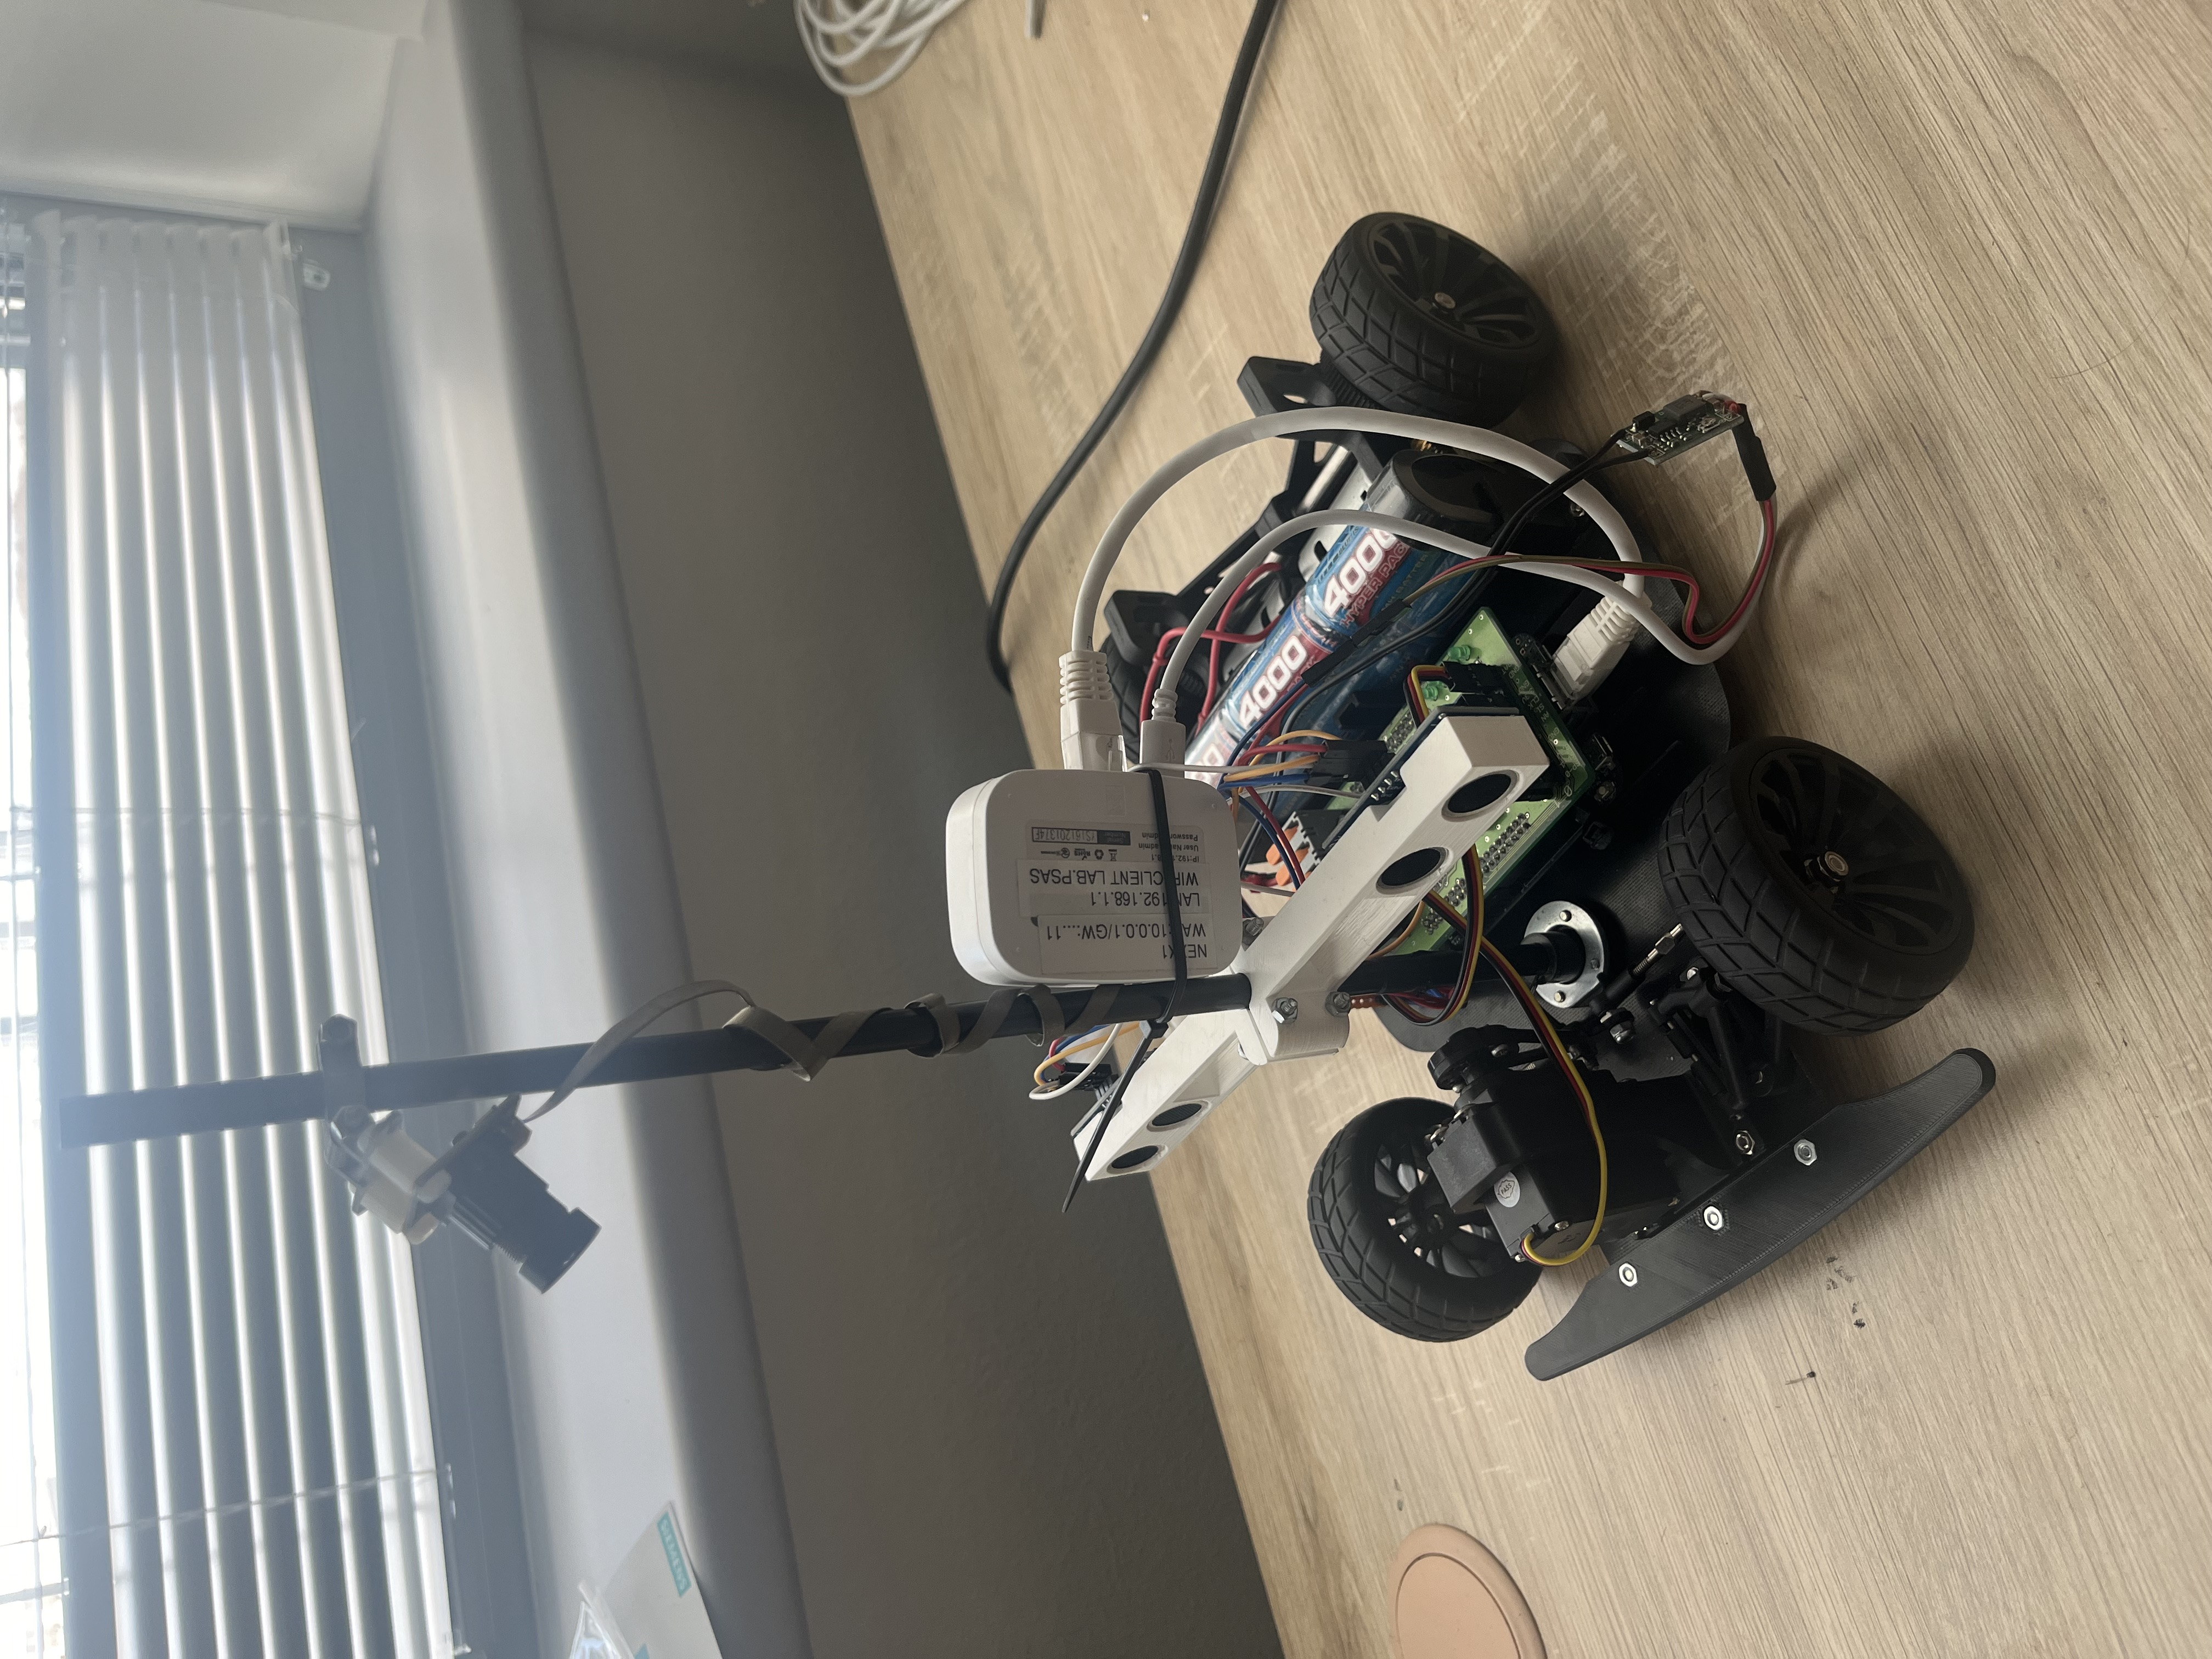
\includegraphics[width=0.45\linewidth, angle=-90]{Figures/car.jpeg}
    \caption{Model auta}
    \label{fig:1}
\end{figure}

\section{Mikrokontroler FRDM-K66F}
\label{sec:FRDM-K66F}

\section{POLI-TFC}
\label{sec:POLI-TFC}

\endinput
